\chapter{Squared-displacement distributions}
\label{app:squared-displacements}

These figures express the test of Section~\ref{sec:component-self-similarity} in
squared metres, using the same observations, weights and six lags. Squaring the
bin edges preserves probability masses, while the exponent doubles according to
Equation~\eqref{eq:squared-displacement-scaling}. This representation adds no
independent evidence for self-similarity.

The shape of a density also changes under this transformation. If a component
magnitude has a finite nonzero density limit $p_Y(0^+)=c$, then
$p_{Y^2}(s)\sim c/(2\sqrt{s})$ as $s\downarrow0$. An approximately straight
descending part of a squared-component density on logarithmic axes can therefore
come from this Jacobian near zero; it is not by itself evidence of a heavy upper
tail. Very small positive bins and exact zero atoms describe numerical observations,
without establishing physical displacement resolution at those scales.

\begin{figure}[htbp]
 \centering
 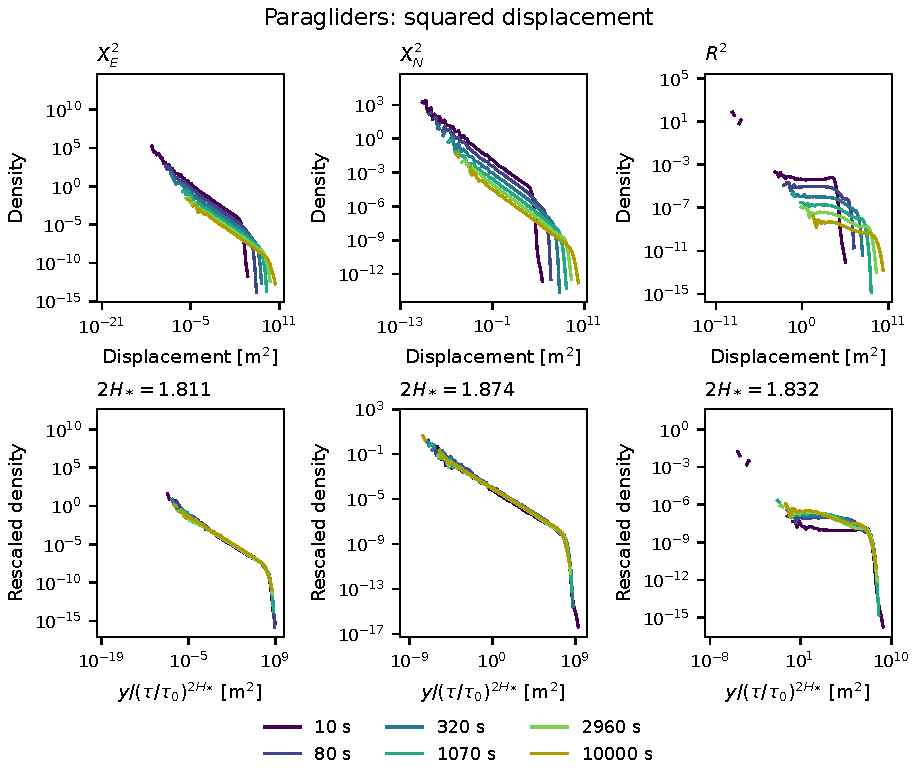
\includegraphics[width=0.95\linewidth]{generated/ch3_squared_laws_para}
 \caption{Paraglider distributions of $X_E^2$, $X_N^2$ and $R^2$. Top: raw densities;
 bottom: rescaling by $(\tau/\tau_0)^{2H_{j,*}}$, with
 $\tau_0=\SI{1000}{\second}$ and the doubled exponents from
 Table~\ref{tab:component-collapse}. Zero atoms are recorded separately.}
 \label{fig:squared-laws-para}
\end{figure}

\begin{figure}[p]
 \centering
 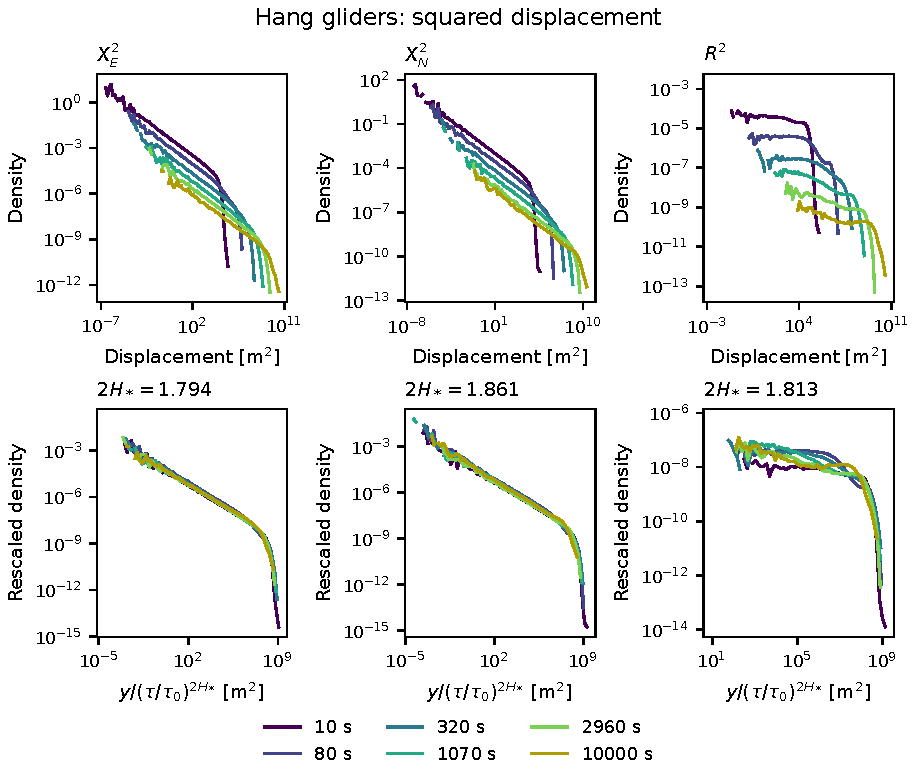
\includegraphics[width=\linewidth]{generated/ch3_squared_laws_hang}
 \caption{The same squared-displacement distributions and rescaling for hang gliders.
 Changes of shape seen for magnitudes remain under the monotone square transformation;
 the corresponding ECDF separation is exactly unchanged.}
 \label{fig:squared-laws-hang}
\end{figure}
